\subsection{Модуль Distributions}

В основе лежит класс \texttt{Distribution}, представленный в виде протокола Python. Это означает, что конкретные классы могут \emph{реализовать} интерфейс \texttt{Distribution}, не наследуясь от общего базового класса. По этой причине почти все поля \texttt{Distribution} экспонируются как свойства (\texttt{@property}); обзор ключевых элементов модуля показан на рис.~\ref{fig:uml-distributions}.

\begin{figure}[htbp]
  \centering
  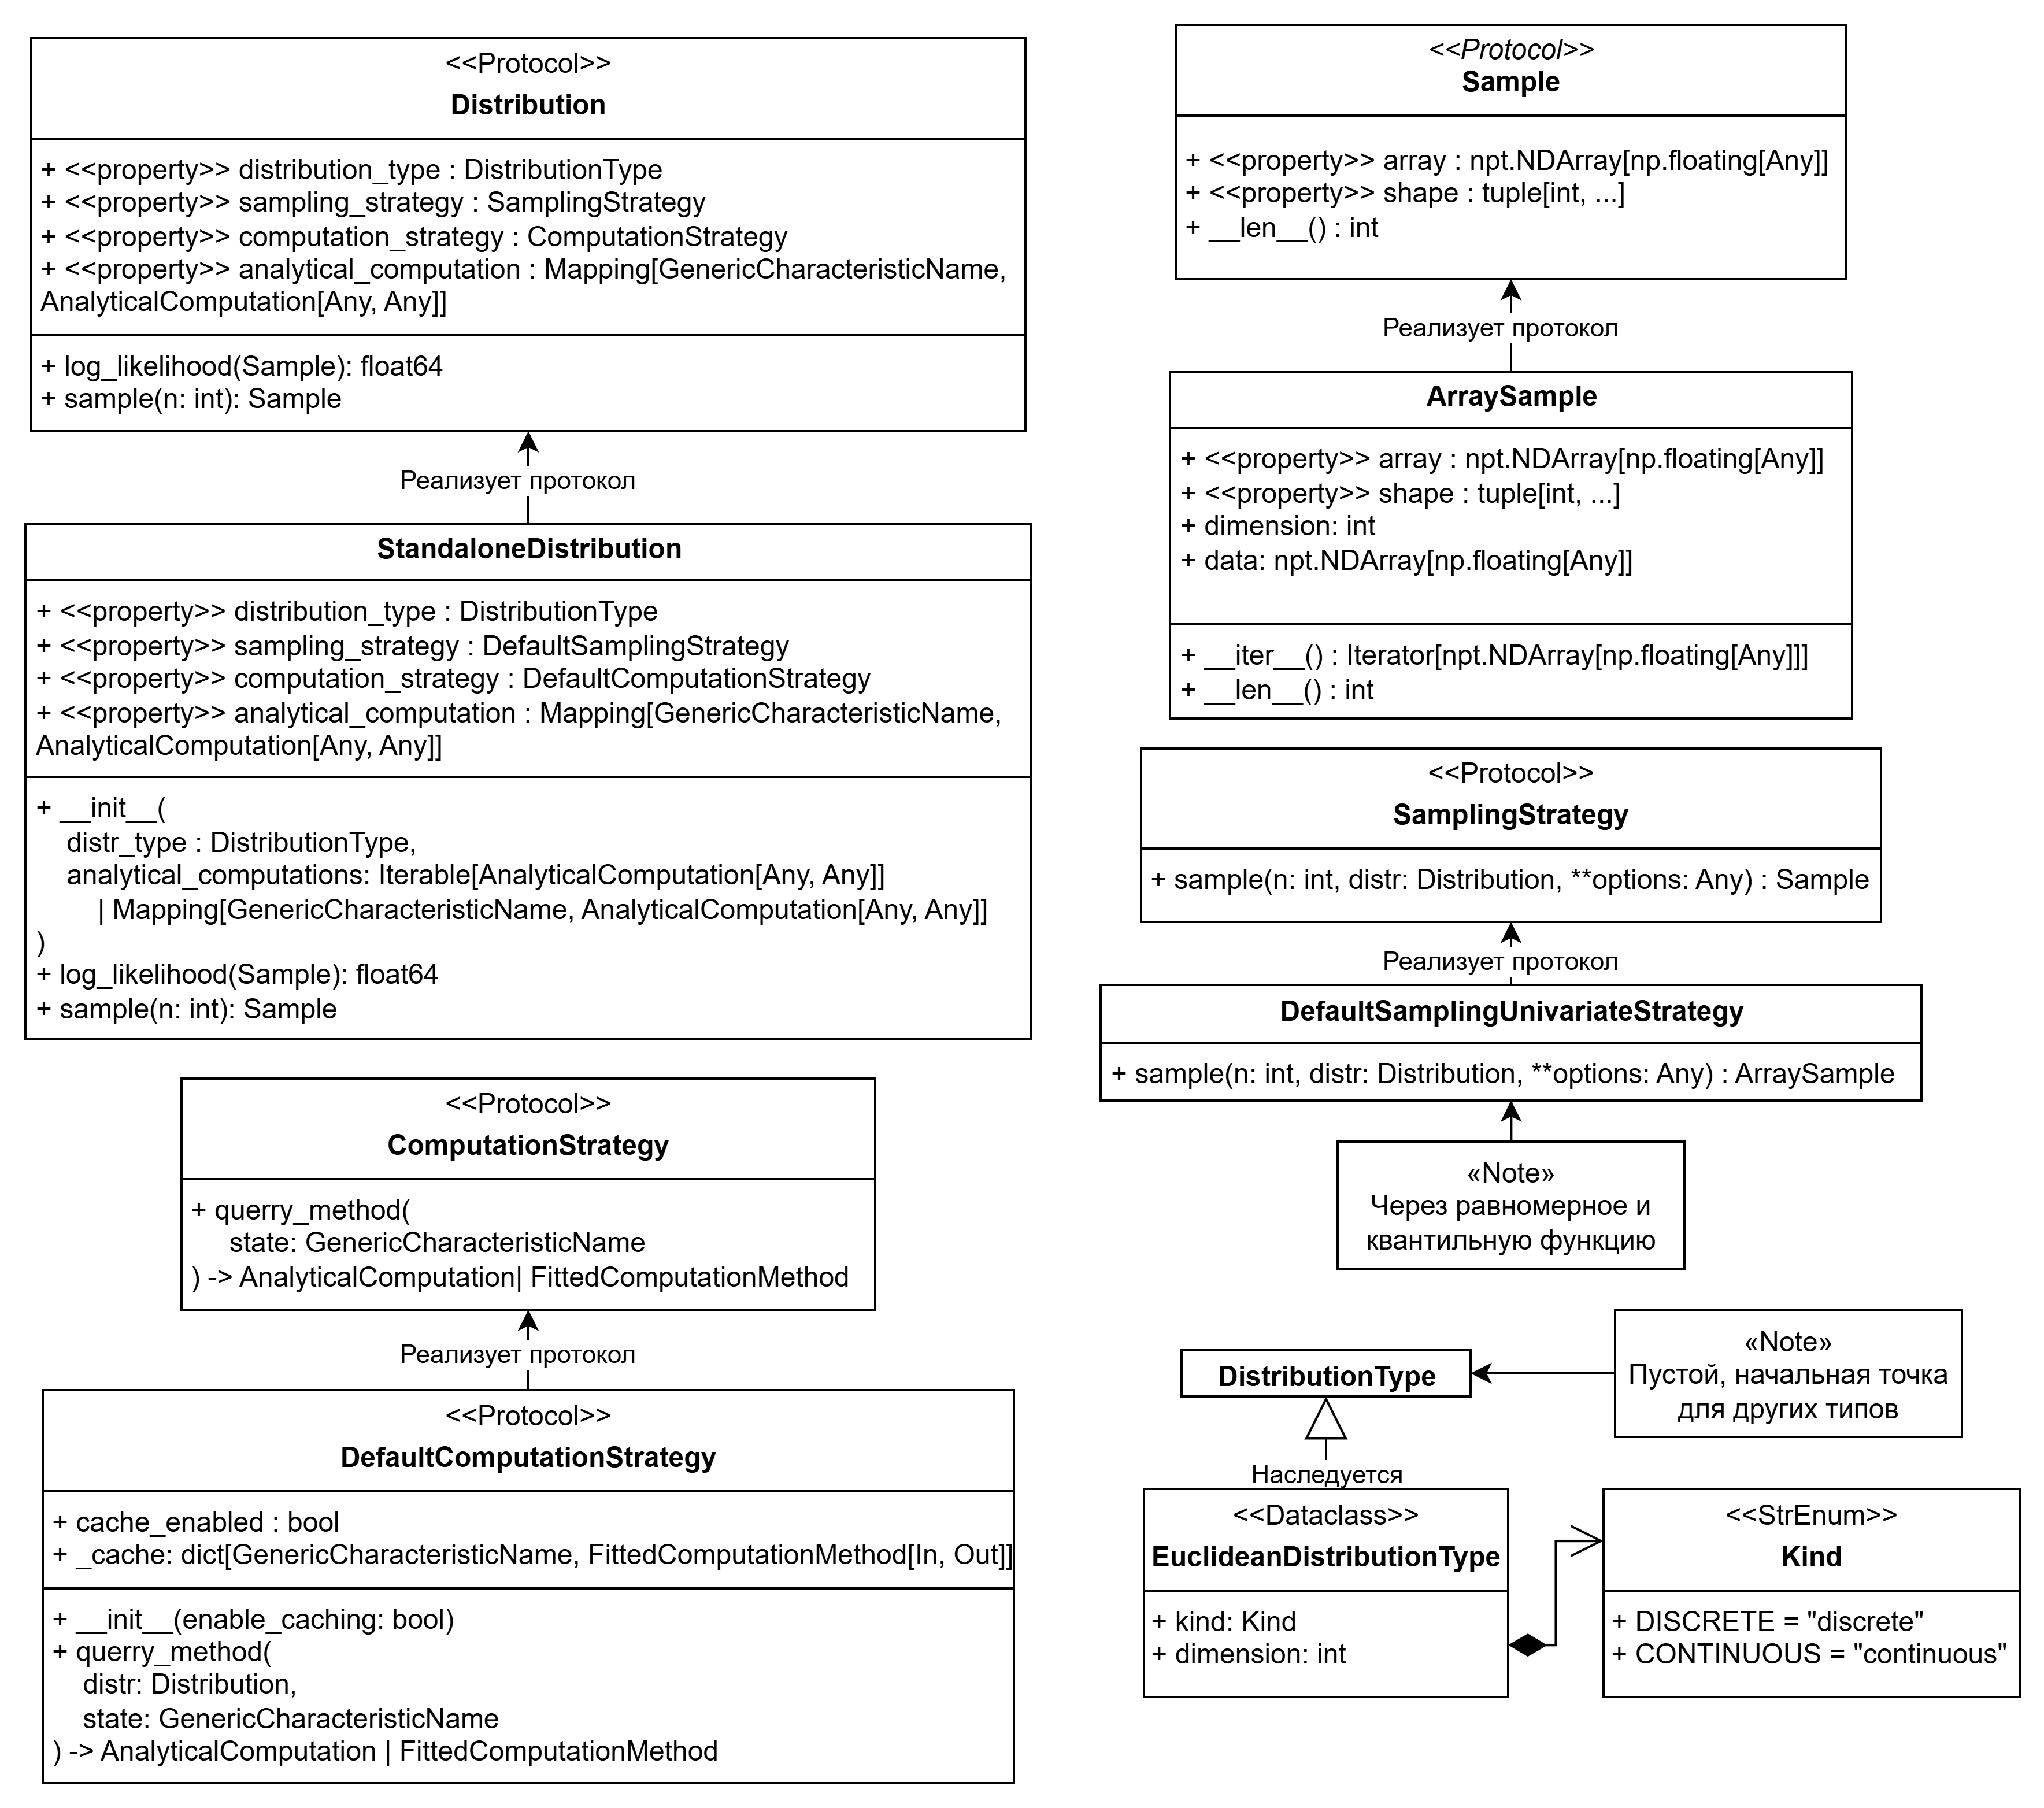
\includegraphics[width=\linewidth]{assets/images/Distrs.png}
  \caption{UML-обзор модуля \texttt{Distributions}: протокол \texttt{Distribution},
  типы \texttt{DistributionType}, стратегии \texttt{SamplingStrategy}/\texttt{ComputationStrategy},
  выборки и базовые реализации по умолчанию.}
  \label{fig:uml-distributions}
\end{figure}

\subsubsection{Тип распределения (\texttt{DistributionType})}

\texttt{DistributionType} — маркерный тип, задающий родовую принадлежность распределения и цепочку наследований признаков, которые принципиально различают семейства распределений. Пример: \texttt{EuclidianDistributionType} со свойствами \texttt{kind} (\texttt{Discrete}/\texttt{Continuous}) и размерностью (евклидово пространство фиксированной размерности). Этот тип не содержит логики вычислений, но определяет область применимости правил преобразований характеристик.

\subsubsection{Стратегии: выборки и вычислений}

\textbf{Стратегия сэмплирования (\texttt{SamplingStrategy}).}
Свойство \texttt{sampling\_strategy} определяет алгоритм генерации выборки из распределения. Стратегия по умолчанию использует квантили (\texttt{ppf}) в сочетании с равномерным распределением для генерации входных вероятностей.

\textbf{Стратегия вычислений (\texttt{ComputationStrategy}).}
Свойство \texttt{computation\_strategy} задаёт политику получения функциональных характеристик. Стратегия принимает решения: выдавать ли характеристику из аналитически заданных, читать её из кэша, либо строить через цепочку преобразований. В реализации по умолчанию применяется следующий порядок:
\begin{enumerate}
  \item проверка наличия аналитической реализации целевой характеристики;
  \item проверка кэша результатов;
  \item поиск пути на графе реестра преобразований (см.~\S\ref{subsec:registry}) и пошаговое вычисление.
\end{enumerate}
Базовая стратегия поддерживает кэширование; кэш прозрачен для вызывающей стороны.

\subsubsection{Аналитические характеристики (\texttt{AnalyticalComputation})}

\texttt{AnalyticalComputation} — это набор функциональных характеристик, заданных в явном (аналитическом) виде и не требующих вывода через другие характеристики. Для каждого конкретного распределения должен существовать хотя бы один такой «якорь», обеспечивающий возможность построения остальных характеристик через реестр преобразований. Здесь \emph{не} подразумевается внешняя «база данных»; речь идёт о \emph{базисе} характеристик самого распределения.

\subsubsection{Выборки и правдоподобие}

\texttt{Sample} и \texttt{ArraySample} — лёгкие обёртки над массивами \texttt{NumPy}, хранящие выборку и метаданные. Для любой реализации \texttt{Distribution} возможно:
\begin{itemize}
  \item сгенерировать выборку согласно \texttt{sampling\_strategy};
  \item вычислить (лог-)\,функцию правдоподобия для этой выборки.
\end{itemize}

\subsubsection{Протокол вычисления характеристики (\texttt{Computation})}

\texttt{Computation} — абстракция вычислительной процедуры для конкретной характеристики (структура на рис.~\ref{fig:uml-computation}):
\begin{itemize}
  \item \texttt{target} — идентификатор целевой характеристики;
  \item \texttt{\_\_call\_\_} — унифицированный вызов вычисления.
\end{itemize}
\texttt{AnalyticalComputation} реализует \texttt{Computation}. Расширение протокола — \texttt{FittedComputationMethod}: оно вводит понятие \emph{источников} (\emph{sources}) — набора характеристик, из которых получается новая. Конкретная реализация \texttt{FittedComputationMethod} заполняет все поля и предоставляет функцию \texttt{func}, задающую фактическое преобразование.

Отдельно выделяется \texttt{ComputationMethod} — абстракция для сложных вычислений, которые не укладываются в сигнатуру вызова \texttt{FittedComputationMethod}. В частности, \texttt{ComputationMethod} намеренно \emph{не} определяет \texttt{fit} как \texttt{\_\_call\_\_}, поскольку его сигнатура отличается. Такое разделение упрощает кэширование и повторное использование результатов.

\begin{figure}[htbp]
  \centering
  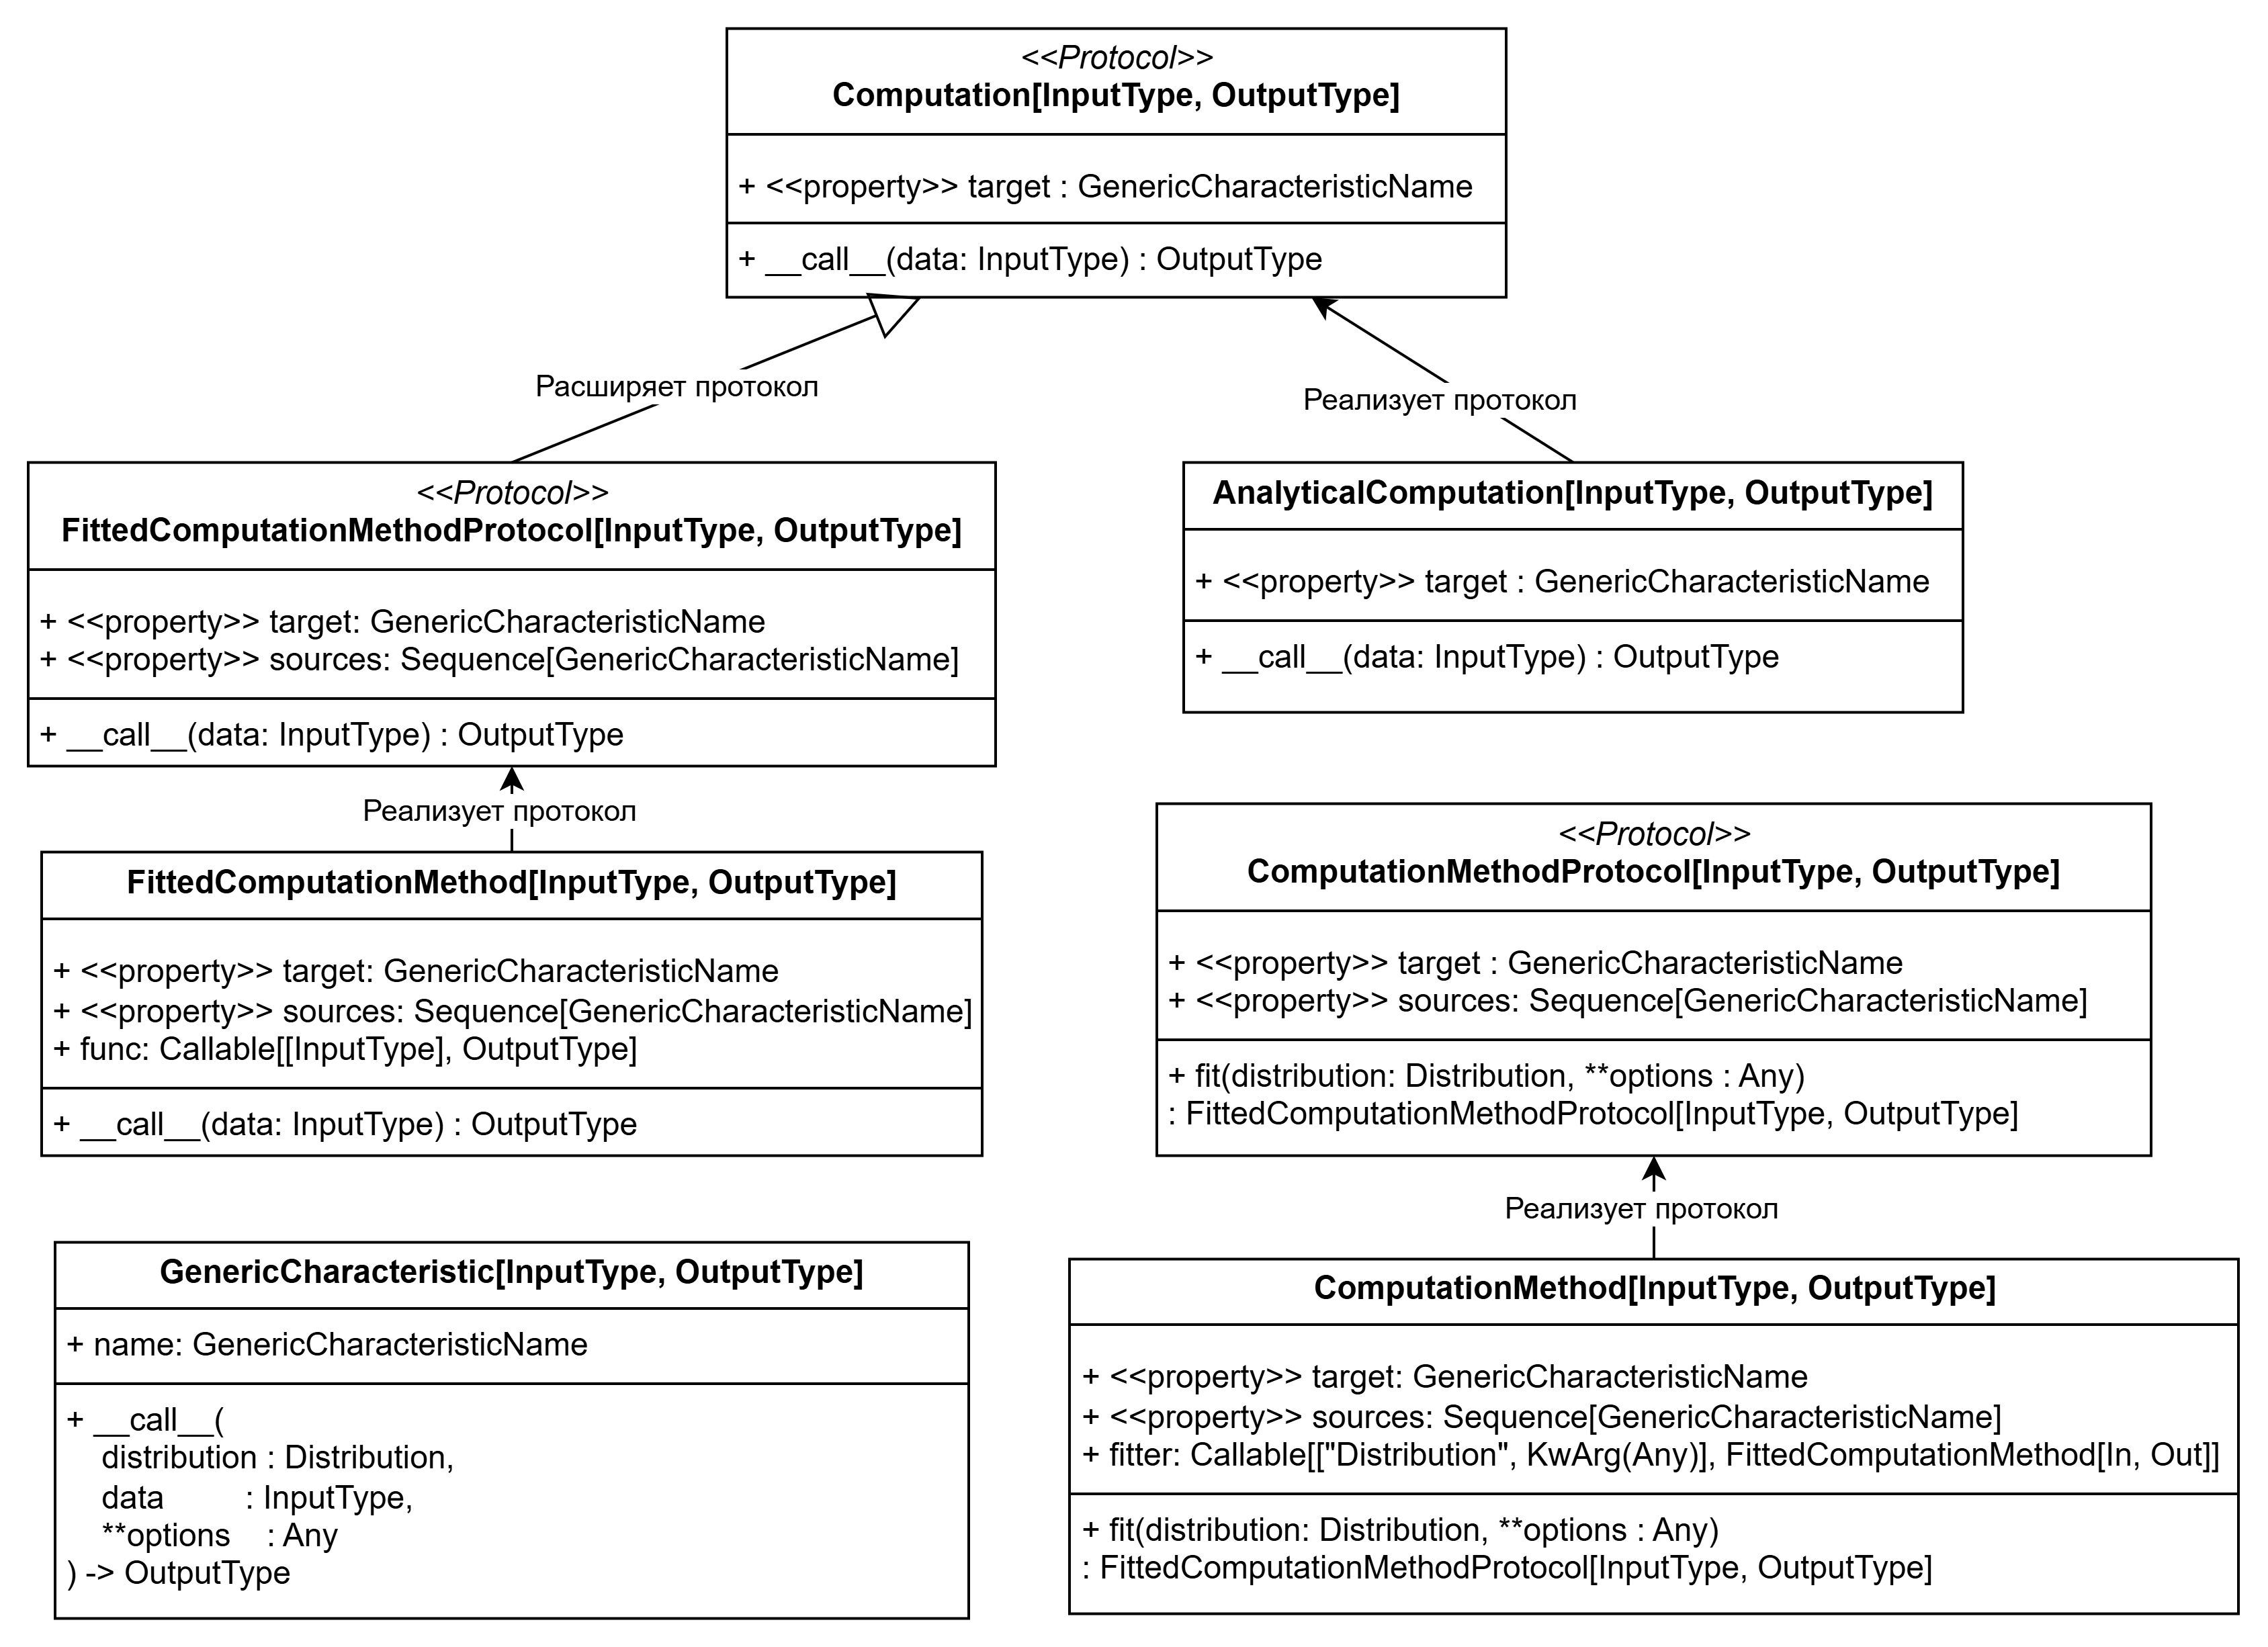
\includegraphics[width=\linewidth]{assets/images/Computation.png}
  \caption{Вычислительная модель: \texttt{Computation}, \texttt{AnalyticalComputation},
  \texttt{FittedComputationMethod} и \texttt{ComputationMethod}; целевая характеристика (\texttt{target}),
  источники (\texttt{sources}) и единый механизм вызова.}
  \label{fig:uml-computation}
\end{figure}

\subsubsection{Имена характеристик и единый механизм вызова}

\texttt{GenericCharacteristicName} — типизированное имя характеристики (не протокол). Вызов для любой характеристики унифицирован:
\begin{enumerate}
  \item у стратегии, закреплённой за распределением, запрашивается подходящий метод для \texttt{target};
  \item полученный метод вызывается над переданными данными.
\end{enumerate}

\textbf{Опции вычислений (\texttt{\textbf{**options}}).}
И \texttt{Characteristic}, и \texttt{ComputationMethod} поддерживают дополнительные параметры, влияющие на ход вычислений. Пример: при восстановлении \texttt{ppf} по \texttt{cdf} можно задать стратегию выбора ветви \texttt{most\_left}/\texttt{most\_right}. Конкретная стратегия \emph{может} проигнорировать опцию, однако пользователь волен подключить собственную стратегию, которая эти опции учитывает.

\subsubsection{Реестр преобразований характеристик}
\label{subsec:registry}

Сердцем архитектуры является \texttt{DistributionTypeRegister} — синглтон, содержащий для каждого \texttt{DistributionType} ориентированный граф переходов между характеристиками (см. рис.~\ref{fig:uml-register}).

\textbf{Структура графа.}
\begin{itemize}
  \item Узлы — имена характеристик.
  \item Рёбра — помечены парами \{имя, \texttt{ComputationMethod}\}. Имя по умолчанию зарезервировано как
  \[
    \texttt{DEFAULT\_COMPUTATION\_KEY} \equiv \texttt{"PySATL\_default\_computation"}.
  \]
  Зарезервированное имя используется для поставляемых реализаций по умолчанию и не рекомендуется для пользовательских методов, чтобы избежать непреднамеренного переопределения.
\end{itemize}

\textbf{Классификация узлов.}
Все характеристики делятся на:
\begin{itemize}
  \item \emph{definitive} — однозначно задающие распределение (например, \texttt{pdf}, \texttt{cdf}, \texttt{ppf});
  \item \emph{indefinitive} — вычислимые по известным характеристикам, но не задающие распределение однозначно (например, математическое ожидание, дисперсия, медиана).
\end{itemize}

\textbf{Инварианты.}
\begin{enumerate}
  \item Подграф \emph{definitive}-узлов всегда связен: из любой definitive-характеристики существует путь в любую другую.
  \item \emph{Indefinitive}-узлы являются стоками: обратных рёбер из них в множество definitive нет.
\end{enumerate}

\textbf{Операции реестра.}
Предоставляются следующие методы управления графом:
\begin{itemize}
  \item \texttt{register\_definitive(name)} — регистрация \emph{единственного} начального definitive-узла в пустом графе. Если попытаться добавить второй исходный узел, сработает проверка инвариантов и будет брошено исключение.
  \item \texttt{add\_bidirectional\_conversion(a, b, method\_ab, method\_ba)} — либо добавляет пару взаимосвязанных узлов в пустой граф, либо присоединяет новый узел к уже существующему связному компоненту (рёбра в обе стороны обязательны, иначе нарушится связность definitive-подграфа).
  \item \texttt{add\_conversion(a, b, method, name?)} — добавляет альтернативный маршрут между уже соединёнными узлами; тем самым поддерживаются множественные реализации преобразования.
  \item Служебные запросы: \texttt{is\_definitive(name)}, \texttt{definitive\_nodes()}, \texttt{indefinitive\_nodes()}, \texttt{all\_nodes()}.
  \item Поиск маршрута: \texttt{find\_path(source, target)} — стандартный \texttt{BFS} по графу, используемый стратегией по умолчанию и доступный пользователю при реализации собственных стратегий.
\end{itemize}

\begin{figure}[htbp]
  \centering
  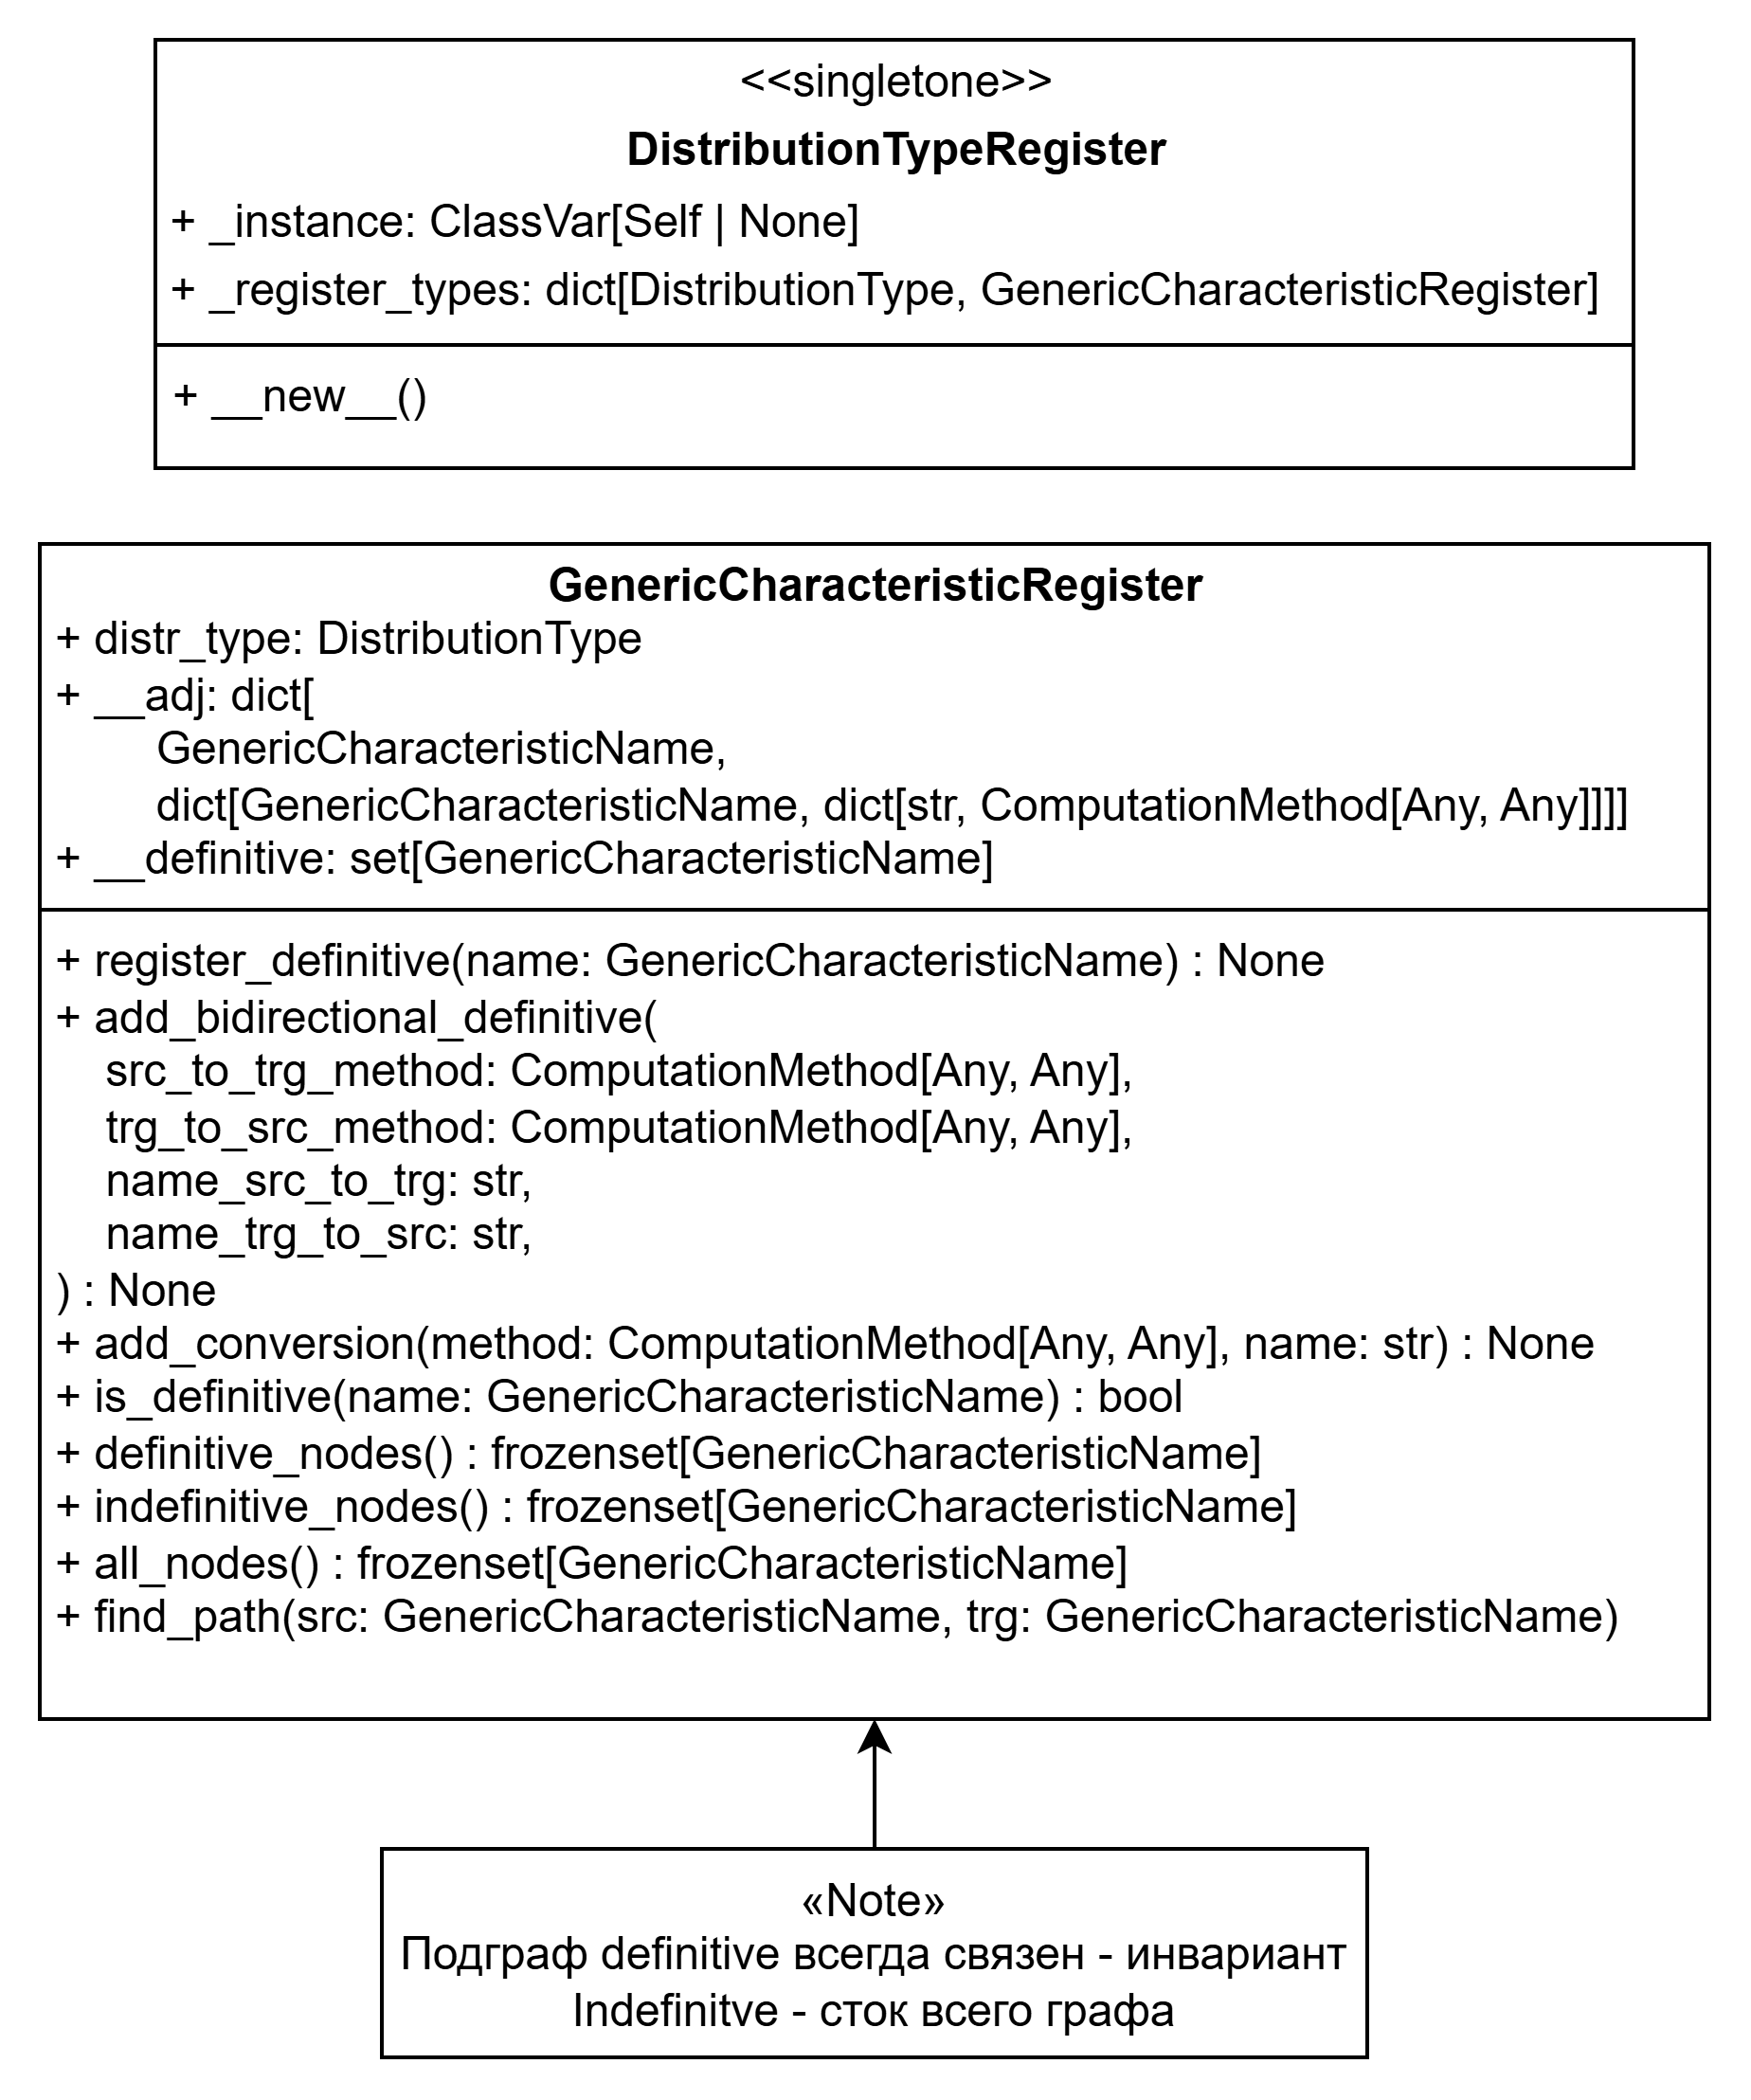
\includegraphics[width=0.5\linewidth]{assets/images/Register.png}
  \caption{Реестр преобразований для типа распределения: \texttt{DistributionTypeRegister}
  и \texttt{GenericCharacteristicRegister} с инвариантами (связность definitive-подграфа,
  отсутствие обратных рёбер из indefinitive).}
  \label{fig:uml-register}
\end{figure}